%%%%%%%%%%%%%%%%%%%%%%%%%%%%%%%%%%%%%%%%%%%%%%%%%%%%%%%%%%%%%

\mainmatter
\setcounter{page}{1}

\lectureseries[\course]{\course}

\auth[\lecAuth]{Lecturer: \lecAuth\\ Scribe: \scribe}
\date{October 13, 2009}

\setaddress

% the following hack starts the lecture numbering at 5
\setcounter{lecture}{4}
\setcounter{chapter}{4}

\lecture{LQG Control with Dynamic Programming}

\section{DP Review}
In discrete time
\begin{align*}
\xi_{t+1} &= f(\xi_t,u_t,w_t) \\
\xi_s &= x \\
J(s,x,u) &= E_w\int_{]s,t-1[}\sum_{t=s}^{T-1}l(x_t,u_t)dt \\
V(s,x,\mu) &= \inf_{\mu\in\mathcal{M}}J(s,x,\mu)
\end{align*}
The optimal control here is feedback control. Using the Dynamic Programming Principle (DPP) and Dynamic Programming Equation (DPE) yields
$$V(t,x) = \min_{u\in\mathcal{U}}\left\lbrace l(x,u) + E_w[V(t+1),f(x,u,w))]\right\rbrace$$

\section{Linear Quadratic Gaussian}
The goal here is to use DP in discrete time to solve the regular LQG problem.
\begin{align*}
\xi_{t+1} &= A\xi_t + Bu_t + \sigma w_t = f(\xi_t,u_t,w_t) \\
\xi_s &= x \in \mathbb{R}^n, ~U=\mathbb{R} \\
\{w_t\} &= \text{ IID }, w_t\sim N(0,Q), ~Q\in\mathbb{R}^{n\times m} \\
J(s,x,\mu) &= E_{w_{]s,T-1[}} \left\lbrace \sum_{t=s}^T \underbrace{\frac{1}{2}\xi_t^T C \xi_t+\frac{1}{2}u_t^TDu_t}_{l} + \underbrace{\frac{1}{2}\xi_t^TF\xi_t}_{\phi} \right\rbrace \\
V(s,x) &= \inf_{\mu\in\mathcal{M}_{s,T-1}}J(s,x,\mu)
\end{align*}
where $C,D,F$ are symmetric positive definite matrices. Then
$$V(T,\cdot) = \frac{1}{2}x^TFx$$

If we assume that $V(t,x) = \frac{1}{2}x^TP_{t+1}x + R_{t+1}$, with $P_{t+1}$ symmetric positive definite and that this is true at $t+1=T$ with $P_T=F$, $R_t=0$, then the DPE is
\begin{align*}
V(t,x) &= \min_{u\in\mathbb{R}^k}\{\frac{1}{2}x^TCx + \frac{1}{2}u^TDU  \\
&+ E_w[\frac{1}{2}(Ax+Bu+\sigma w)^TP_{t+1}(Ax+Bu+\sigma w) + R_{t+1}]\} \\
&= \frac{1}{2}x^TCx + R_{t+1} \\
&+ \min_u \{\frac{1}{2}u^TDu + \frac{1}{2}(Ax+Bu)^TP_{t+1}(Ax+Bu) \\
&+ 2\cdot\frac{1}{2}E_w[(Ax+Bu)^TP_{t+1}\sigma w] + \frac{1}{2}E_w[w^T\sigma^TP_{t+1}\sigma w]\} \\
&= \frac{1}{2}x^TCx + R_{t+1} + \frac{1}{2}E_w[w^T\sigma^TP_{t+1}\sigma w] \\
&+ \min_u \{ \frac{1}{2}u^TDu + \frac{1}{2}(Ax+Bu)^TP_{t+1}(Ax+Bu) \\
&+ (Ax+Bu)^TP_{t+1}\sigma E_w[w] \} \\
&= \frac{1}{2}x^TCx + R_{t+1} + \frac{1}{2}E_w[w^T\sigma^TP_{t+1}\sigma w] \\
&+ \min_u \left\lbrace \frac{1}{2}u^TDu + \frac{1}{2}(Ax+Bu)^TP_{t+1}(Ax+Bu) \right\rbrace \\
\end{align*}
where the last equality occurs because $E_w[w]=0$ and at the second and third equalities all terms that are not a function of $u$ were pulled out in front.

\textit{Exercise:} Find a closed form expression for $E[w^T\sigma^TP_{t+1}\sigma w]$. Use $Q=\Lambda^T\Sigma\Lambda$ or $P_{t+1} = S_{t+1}^T\Sigma_{t+1}S_{t+1}$. These will result in an equation with the trace of a matrix and the Frobenius norm.

Continuing on we have
\begin{align*}
R_t = R_{t+1} + \frac{1}{2}E_w[w^T\sigma^TP_{t+1}\sigma w]
\end{align*}
\begin{align*}
&\Rightarrow V(t,x) = \frac{1}{2}x^TCx + R_t \\
&\qquad + \min_u\{ \underbrace{\frac{1}{2}u^TDu + \frac{1}{2}(Ax)^TP_{t+1}Ax + \frac{1}{2}u^TB^TP_{t+1}Bu + (Ax)^TP_{t+1}Bu\}}_{G(u)}
\end{align*}

\textit{Exercise:} Find the grandient of $\frac{1}{2}u^TAu$ and $B^Tu$.

This leads to
\begin{align*}
\nabla G &= Du + B^TP_{t+1}Bu + B^TP_{t+1}Ax = 0 \\
(D+B^TP_{t+1}B)u &= -B^TP_{t+1}Ax \\
u &= -(D+B^TP_{t+1}B)^{-1}B^TP_{t+1}Ax \doteq K_tx \doteq \mu_t(x)
\end{align*}
where $\mu_t(x)$ is our feedback controller. The first equation corresponds to (3.10-8) in Kirk\footnote{"Optimal Control Theory: An Introduction" by Donald E. Kirk.} and the third equation corresponds to (3.10-10) in Kirk. Then we have that
$$V(t,x) = \frac{1}{2}x^TP_tx + R_t$$
with
$$P_t = C+ K_t^TDK_t + (A+BK_t)^TP_{t+1}(A+BK_t)$$
and by induction $V$ has this form $\forall t\leq T$. The equation for $V(t,x)$ corresponds to (3.10-11) in Kirk.

\section{Convex Analysis}
\begin{definition}
$\mathcal{C}\in\mathbb{R}^n$ is convex if
$$\lambda x + (1-\lambda)y \in \mathcal{C} ~\forall x,y\in\mathcal{C}, ~\forall \lambda\in[0,1]$$
This can be seen by noticing that
$$\{\mathcal{Z}\in\mathbb{R}^n | z=\lambda x+(1-\lambda)y, ~\lambda\in[0,1]\}$$
is a line segment from $x\to y$ as shown in Figure \ref{fig:05convex}.
\end{definition}

\begin{figure}[ht!]
	\centering
	\subfloat[Convex set.]{
		\label{fig:05convexSet}\includegraphics[width=0.3\textwidth]{images/05convexSet}
	} \hfill
	\subfloat[Not a convex set.]{
		\label{fig:05notConvexSet}\includegraphics[width=0.3\textwidth]{images/05notConvexSet}
	}
	\caption{\subref{fig:05convexSet} Example of a convex set and \subref{fig:05notConvexSet} example of a set that is not convex.}
	\label{fig:05convex}
\end{figure}

\begin{definition}
Given a function $f:\mathbb{R}^n\to\mathbb{R}$ then the epigraph of that function is
$$\text{epi}[f] \doteq (x,z)\in\mathbb{R}^{n+1} \text{ s.t. } z\geq f(x)$$
Figure \ref{fig:05epigraph} shows that the epigraph is the set of points above and including the curve described by $f$.
\end{definition}

\begin{figure}[ht!]
	\centering
	\includegraphics[width=.4\textwidth]{images/05epigraph}
	\caption{The epigraph of $f$ is the shaded area above $f$ including the curve.}
	\label{fig:05epigraph}
\end{figure}

\begin{definition}
A function $f:\mathbb{R}^n\to\mathbb{R}$ is convex if $\text{epi}[f]$ is a convex set.
\end{definition}

\begin{theorem}
$f$ is convex $\Leftrightarrow f(\lambda x + (1-\lambda)y)\leq \lambda f(x) + (1-\lambda)f(y) ~\forall x,y\in\mathbb{R}^n, ~\forall \lambda\in[0,1]$.
\end{theorem}
Figure \ref{fig:05convexGeoProof} gives an illustration.
\begin{proof}
This proof is for the if portion, not the only if portion. Let $x,y\in\mathbb{R}^n, ~\lambda\in[0,1]$. Since $f$ is convex we know that $\text{epi}[f]$ is a convex set such that
\begin{align*}
&\left(\begin{array}{c} x \\ f(x) \end{array}\right), ~\left(\begin{array}{c} y \\ f(y) \end{array}\right) \in \text{epi}[f] \\
&\therefore \lambda\left(\begin{array}{c} x \\ f(x) \end{array}\right) + (1-\lambda)\left(\begin{array}{c} y \\ f(y) \end{array}\right) \in \text{epi}[f] \\
&\Rightarrow \left(\begin{array}{c} \lambda x+(1-\lambda)y \\ \lambda f(x) + (1-\lambda)f(y) \end{array}\right) \in \text{epi}[f] \\
&\Rightarrow \lambda f(x) + (1-\lambda)f(y) \geq f(\lambda x + (1-\lambda)y)
\end{align*}
\end{proof}

\begin{figure}[ht!]
	\centering
	\includegraphics[width=.5\textwidth]{images/05convexGeoProof}
	\caption{A curve $f$ is convex if it is as shown.}
	\label{fig:05convexGeoProof}
\end{figure}

It is nice to optimize convex functions because there is only a single global minimum and no local minimums to get trapped in.

\begin{theorem}
If $f$ is convex and real-valued then $f$ is continuous.
\end{theorem}

\begin{theorem}
If $f$ is continuous on a compact set then a minimum exists.
\end{theorem}

\begin{definition}
$f\to\infty$ as $x\to\infty$ if given $M<\infty \exists R<\infty$ such that $f(x)\geq M ~\forall |x|\geq R$.
\end{definition}

\begin{theorem}
$f:\mathbb{R}^n\to\mathbb{R}$ is convex if $f\to\infty$ as $x\to\infty$ then $\exists \bar{x}\in\mathbb{R}^n$ such that $f(\bar{x})\leq f(x) ~\forall x$.
\end{theorem}

\begin{theorem}
If $f\in\mathbb{C}^2$ and $\frac{d^2f}{dx^2}$ is positive definite then $f$ is convex.
\end{theorem}

\begin{theorem}
\label{th:sumConvex}
If $f_1$ and $f_2$ are convex then $f_1+f_2$ is convex.
\end{theorem}

\begin{proof}
Let $g(x) \doteq f_1(x) + f_2(x) ~\forall x$ and let $\lambda\in[0,1]$.
\begin{align*}
g(\lambda x + (1-\lambda)y) &= f_1(\lambda x+(1-\lambda)y) + f_2(\lambda x+(1-\lambda)y) \\
&\leq \lambda f_1(x) + (1-\lambda)f_1(y) + \lambda f_2(x) + (1-\lambda)f_2(y) \\
&= \lambda g(x) + (1-\lambda)g(y)
\end{align*}
\end{proof}

\begin{theorem}
\label{th:cfxconvex}
If $f$ is convex, $c\geq 0$ and $f(x)\geq 0 ~\forall x$ then $cf(x)$ is convex.
\end{theorem}

\begin{proof}
Let $g(x)=cf(x)$. Then
\begin{align*}
g(\lambda x+(1-\lambda)y) &= cf(\lambda x+(1-\lambda)y) \\
&\leq c\lambda f(x) + c(1-\lambda)f(y) \\
&= \lambda g(x) + (1-\lambda)g(y)
\end{align*}
\end{proof}

\begin{theorem}
\label{th:maxconvex}
If $f_1$ and $f_2$ are convex then $f_1\oplus f_2$ is convex.
\end{theorem}

\begin{proof}
See Figure \ref{fig:05convexOplusProof} for a geometrical proof.
\end{proof}

\begin{figure}[ht!]
	\centering
	\includegraphics[width=.4\textwidth]{images/05convexOplusProof}
	\caption{Geometrical proof showing region of convexity for two functions.}
	\label{fig:05convexOplusProof}
\end{figure}

\begin{theorem}
\label{th:argconvex}
If $f$ is convex and $a\in\mathbb{R}^n$ then $g(x)\doteq f(x+a)$ is convex.
\end{theorem}

\begin{theorem}
\label{th:randconvex}
If $f$ is convex and $Z$ is a RV with range in $\mathbb{R}^n$ then $E[f(x+Z)]$ is convex.
\end{theorem}

\begin{proof}
\begin{align*}
E[f(\lambda x+(1-\lambda)y) + Z] &= E[f(\lambda(x+Z) + (1-\lambda)(y+Z))] \\
&\leq E[\lambda f(x+Z) + (1-\lambda)f(y+Z)] \\
&= \lambda E[f(x+Z)] + (1-\lambda)E[f(y+Z)]
\end{align*}
\end{proof}

\section{Inventory Control}
Let $\xi_t$ be current inventory, $u_t$ be the amount of new inventory to purchase, $w_t$ a radom process involving selling inventory and let these three variables be IID. Let $\xi_{t+1} = \xi_t+u_t+w_t$ and the values of $c,p,h>0$ be constants. Then the cost function can be written as
\begin{align*}
J(s,x,\mu) =& E_{w_{]s,T-1[}} \\
&\left[\sum_{t=s}^{T-1}cu+p\max[0,-(\underbrace{\xi_t+u_t+w_t}_{\xi_{t+1}})] + h\max[0,\underbrace{\xi_t,u_t,w_t}_{\xi_{t+1}}] \right]
\end{align*}
where the first $\xi_{t+1}$ represents the cost of having backlogged orders and the second one represents the cost of storing excess inventory. To determine the optimal amount of inventory to purchase (or our system input) we can use DP with $\phi=0$ to mean that no terminal cost exists. This means that $V(t,x)=0$ and gives
\begin{align*}
V(t,x) &= \min_{u\geq 0}E_w[cu+p\max(0,-\xi_{t+1})) \\
&+ h\max(0,\xi_{t+1}) + V(t+1,x+u+w)] \\
&\doteq min_{u\geq 0}H(x,u)
\end{align*}
From here we can use convex analysis since $cu$, $x+u+w$ and $-(x+u+w)$ are all convex in $u$. Suppose $V(t+1,\cdot)$ is convex where the $\cdot$ represents the state. Then by Theorem \ref{th:argconvex} we have that $V(t+1,x+u+w)$ is convex in $u$. Theorems \ref{th:cfxconvex} and \ref{th:maxconvex} show that $p\max(0,-(x+u+w))$ and $h\max(0,x+u+w)$ are convex in $u$. Then Theorem \ref{th:randconvex} means that $H(x,u)$ is convex in $u$.

Let $y=u+x$, then
\begin{align*}
&\min_{y\geq x}\{ c(y-x)+pE[\max(0,-(y+w))] \\
&+ hE[\max(0,y+w)] + E[V(t+1,y+w)]\}
\end{align*}
is convex in $y$. Let a minimum exist at $\bar{y}$. Then, if $\bar{y}\geq x$ then choose $w_t(x) = \bar{g}-x$ which represents buying new inventory. If $\bar{y}<x$ then choose $w_t(x)=0$ which represents no action. This implies that no control exists when selling inventory because it is a RV. Then
$$V(t,x) = \begin{cases} H(\bar{y}), & x<\bar{y} \\ H(x), & x>\bar{y} \end{cases}$$
$V(t,\cdot)$ is convex follows by induction.

%%%%%%%%%%%%%%%%%%%%%%%%%%%%%%%%%%%%%%%%%%%%%%%%%%%%%%%%%%%%%